\documentclass[11pt,twoside,a4paper]{mr}%two-page printing
\usepackage[utf8]{inputenc}

\usepackage{hyperref}
\usepackage{graphicx}
\usepackage{color}
\usepackage{array}
\usepackage{eurosans}
\usepackage{amsmath,amssymb,amsfonts}
\usepackage{mathtools}

% Title Page
\title{\bfseries Bicing}
\author{\textit{\textbf{Tomas Barton}} and \textit{\textbf{Mauro Donadeo}}}


\begin{document}
\maketitle

% \begin{abstract}
% \end{abstract}

\chapter{Introduction}
The aim of this project is to provide an program which would help the provider of local bicing service\footnote{Bicing Barcelona -- \url{http://www.bicing.com}} with distribution of bikes to approach to an ideal state, when each user of this service would find a bike when he needs it. 

\section{About Bicing}
The Bicing project is quite new in Barcelona (started in 2007\cite{bicingw}), but after few months it became very popular. Owner of a special card, which can be purchased for 30~\euro \, per year, can rent a bike from a station for free, if he returns this bike to some station in a half an hour. Otherwise he pays a few cents for each hour until the bike is returned. 

\begin{figure}[ht]
\begin{center}
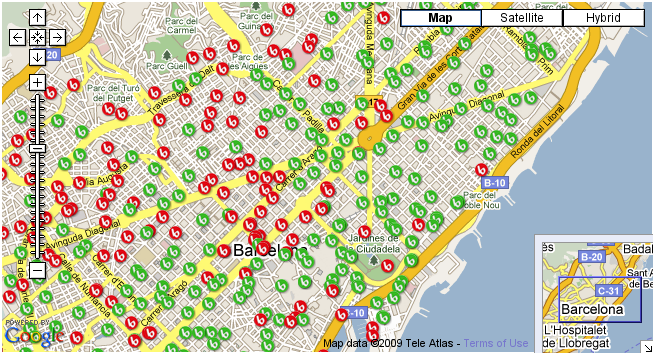
\includegraphics[width=\textwidth]{images/bicing_map.png}
\caption{Map of bicing stations in Barcelona -- red stations are without bikes}
\label{img:bicing_map}
\end{center}
\end{figure}

Nowadays there are more than 400\footnote{418 stations at 12 October 2009} bike stations in Barcelona, the highest concentration of bike stations is of course in centre of city. Usually each station has from 20 up to 30 stands for bikes. In the very center they are placed quite close to each other.

\section{Our task}
With usage of \textbf{\textsl{F}} vans we are supposed to optimize distribution of bikes, so that as many customers as possible will find a disposable bike at time when they need it.

Implementation has been done in Java, we took advantage of AIMA framework\cite{aima}, which contains most of algorithms commonly used for  searching state space.

\section{Complexity of problem}
As long as we have to search just for solution of this problem for upcoming hour, size of state space is significantly reduced. When we display all possible states of this problem as a n-ary tree, we get not really deep tree -- this is exactly the number of maximum moves we can do and that is \textbf{\textsl{F}}, but this tree can have a huge branching factor. 

Number of different moves between stations can be approximately computed as:

\begin{align}
 moves &= F * 2 * \left( {\begin{array}{*{20}c}
n \\
2 \\
\end{array}} \right)
\end{align}

\begin{tabbing}
where     \= \(n\) -- is number of stations\\
	\> \(F\) -- number of vans
 \end{tabbing}

We are looking for different pairs of stations and we can move bikes in both directions, so that we multiply combination by 2. In this formula we do not consider moves of different number of bikes between same stations. 

\begin{align*}
 moves &= F * 2 * \left( \frac{n!}{2* (n-2)!} \right) \\
       &= F * 2 * \frac{n*(n-1)(n-2)!}{2*(n-2)!} \\
       &= F * n * (n-1) 
\end{align*} 

So that polynomial complexity of this problem seems to be:

\begin{align}
 T(n) &= O( k* n^2 ) = O( n^2 )
\end{align}



\chapter{Implementation}
\section{State representation} 
Each state must contain information about distribution of bikes over all stations. So that we have to keep:
\begin{itemize}
\item current number of bikes at the station
\item number of bikes that is going to be at station in an hour 
\item moves how to reach this state (from empty state)
\end{itemize}
These information are different for each state, moreover we have other information which we need but they are same for every state:
\begin{itemize}
 \item number of stations
 \item coordinates of stations
 \item expected demand for bikes in upcoming hour
\end{itemize}


\section{Operators}
For the sake of creating new state we have implemented a set of operators. Firstly we have operator \texttt{addMove} for moving bikes from one station to another. It is quite clear that this operator can be used only when we have some not used bikes at a station. A bit more complicated case is when we load bikes at one station and unload them at two other stations, for this purpose we have \texttt{doubleMove} operator.

Secondly there is operator for altering already done move, which is called \texttt{changeMove} and we allowed changing number of bikes which are going to move and the destination. This operator checks availability of requested bikes at the station, in case that the number of bikes is not at the station, operator returns \texttt{false}. There is also possibility of changing source station but there might not be any bikes available and furthermore this action can be done by combination of \texttt{removeMove} and \texttt{addMove} (with requested source station).

Lastly we have already mentioned operator \texttt{removeMove} which delete move and return bikes to original location.

Here is a sort overview of all operators:
\begin{description}
 \item[addMove] simply moves given number of bikes from one station to another
\item[doubleMove] loads \( a + b \) bikes at one station and unload \(a\) bikes at first station and \(b\) bikes at second station
\item[changeMove] alter number of bikes or destination of this move
\item[removeMove] deletes specified move
 \end{description}

\section{Heuristic functions}
Heuristic function is supposed to evaluate state, so that searching algorithm can unambigously determine which state is better. 

\subsection*{Version 1}
Firstly, we have to take in consideration number of unsatisfied demand of bikes. If there are no bikes needed, or the demand is satisfied, the value of heuristic function would be 0. We are trying to minimize this formula: 

\begin{align}
 h_1 &=\sum\limits_{i=0}^{numStations} not\_satistifed\_demand_i
\end{align}

Let us take into consideration situation when we have 4 stations and bike are all bikes are located only on first station, as it is described in table \ref{t:ex1a}.


\begin{table}[!t]
\renewcommand{\arraystretch}{1.1}
\label{t:ex1a}
\begin{center}
\begin{tabular}[t]{|r|r|r|r|}
\hline
\bf Station \# & \bf Not used & \bf Next &\bf Demand\\ \hline\hline
\sl1 & 10 & 10 & 0\\ \hline
\sl2 & 0 & 0 & 0\\ \hline
\sl3 & 0 & 0 & 2\\ \hline
\sl4 & 0 & 0 & 8\\ \hline
\end{tabular}
\end{center}

\caption{Initial state with heristic value \(h_1= 10.0\)}
\end{table}

The output of this function seems to be correct, if we move 4 bikes to station number~4, we would lower heuristic value to 6, but if we made nonsense move with other~6 bikes to station~2 (as is shown in \ref{t:ex1b}), the value of heuristic function would be the same, so that we introduced version~2.

 \begin{table}[!t]
\renewcommand{\arraystretch}{1.1}

\label{t:ex1b}
\begin{center}
\begin{tabular}[t]{|r|r|r|r|}
\hline
\bf Station \# & \bf Not used & \bf Next &\bf Demand\\ \hline\hline
\sl1 & 0 & 10 & 0\\ \hline
\sl2 & 0 & 6 & 0\\ \hline
\sl3 & 0 & 0 & 2\\ \hline
\sl4 & 0 & 4 & 8\\ \hline
\end{tabular}
\end{center}
\caption{Initial state with heristic value \(h_1= 6.0\)}
\end{table}

\subsection*{Version 2}
This heuristic function proceed from version 1 however it takes into account also bikes which are not going to be used in next hour. Like in previous version we are trying to minimize \textsl{h\_2} value.

\begin{align}
 h_2 &=\sum\limits_{i=0}^{numStations} not\_satistifed\_demand_i + not\_used\_bikes\_in\_next\_hour_i
\end{align}

This function would penalize previously shown example but in some cases it would not be possible to reach score 0.0 for best solution.

\sub

\section{Sucessor function}


\chapter{Experiments}

\chapter{Conclusion}

\clearpage
\begin{thebibliography}{9}
\bibitem{aima}{\em Stuart Russell and Peter Norvig:}{\bf Artificial Intelligence: A Modern Approach}
		\url{http://aima.cs.berkeley.edu/} \\
		{Downloaded java implementation of algorithms (AIMA framework) from repository \url{http://code.google.com/p/aima-java/} by Ravi Mohan. Date of publication: October 3, 2009. \\
		Date retrieved: October 12, 2009. }
\bibitem{bicingw}{\em Wikipedia: }{\bf Bicing}
\url{http://en.wikipedia.org/wiki/Bicing}\\
{Date visited: October 27, 2009}


\end{thebibliography}



\end{document}          
